%**************************************************************
% Lab 09: ROM
%**************************************************************
\chapter{ROM}\label{Lab09}

\section{Purpose}

This lab introduces students to \acf{ROM} and builds a fun application: The Magic 8-Ball. This was a toy that was developed in the 1950s and was popular throughout the 1960s. It was a small sphere with the markings of an 8-ball. If the user ``asked it a question'' and then turned the ball upside down the answer would magically appear in a small window on the bottom of the ball.

\section{Procedure}

Start a new \LE project and create a subcircuit named \lstinline[columns=fixed]|Magic_8_Ball|. Open that circuit and place a ROM (\textit{Memory} library) device near the center of the drawing canvas. Set the ROM properties for an \textit{Address Bit Width} of 12 and a \textit{Data Bit Width} of 8.

\begin{figure}[H]
	\centering
	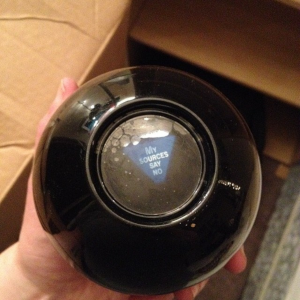
\includegraphics[width=\maxwidth{.95\linewidth}]{gfx/09-01}
	\caption{Placing ROM}
	\label{fig:09-01}
\end{figure}

A ROM stores data that is accessed by setting an address on the inputs at the top left of the device and then reading the contents of that address on the 8-bit bus on the right side of the device. By attaching a counter to the ROM address port several consecutive addresses can be ``stepped through'' to output a message. Attach a Counter (\textit{Memory} library) with 12 Data Bits to the address port of the ROM, as in Figure \ref{fig:09-02}.

\begin{figure}[H]
	\centering
	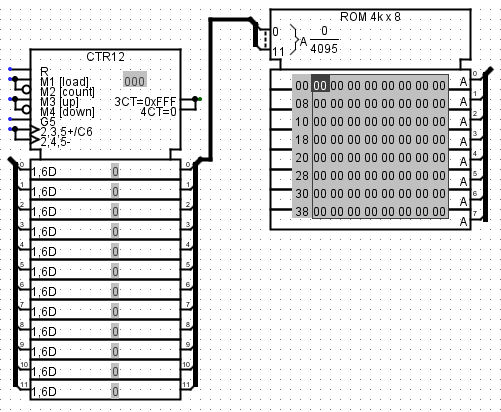
\includegraphics[width=\maxwidth{.95\linewidth}]{gfx/09-02}
	\caption{ROM With Counter}
	\label{fig:09-02}
\end{figure}

According to Wikipedia\footnote{\url{https://en.wikipedia.org/wiki/Magic_8-Ball}}, the Magic 8-Ball featured 20 sayings: 

\begin{verbatim}
 1 001 It is certain
 2 00f It is decidedly so
 3 022 Without a doubt
 4 032 Yes definitely
 5 041 You may rely on it
 6 054 As I see it yes
 7 064 Most likely
 8 070 Outlook good
 9 07d Yes
10 081 Signs point to yes
11 094 Reply hazy try again
12 0a9 Ask again later
13 0b8 Better not tell you now
14 0d1 Cannot predict now
15 0e4 Concentrate and ask again
16 0fe Do not count on it
17 111 My reply is no
18 120 My sources say no
19 132 Outlook not so good
20 146 Very doubtful
\end{verbatim}

The Magic 8-Ball simulator built in this lab uses those same 20 saying. In the above chart, each saying is numbered and the start point in ROM for each saying is also noted. Thus, saying one starts on ROM byte 000, saying two starts on ROM byte 00f, saying three starts on ROM byte 022, and so forth.

The content of the ROM device must be loaded before it can be used and that content is provided in \emph{\texttt{Lab09\_ROM.txt}} accompanying this lab. To load the ROM device, click it one time and then click the ``(click to edit)'' link in its properties panel. In the ROM editor window that pops up, click the ``open'' button and navigate to the ROM memory file. Click ``close window'' to load the ROM device and make it ready for service.

The start point for each saying, as indicated on the above table, is stored in Constants (\textit{Wiring} library) and a Mux (\textit{Plexers} library) with five select bits is used to channel the start byte in ROM Memory for a specific message to the counter. Figure \ref{fig:09-03} illustrates the circuit at this point.

\begin{figure}[H]
	\centering
	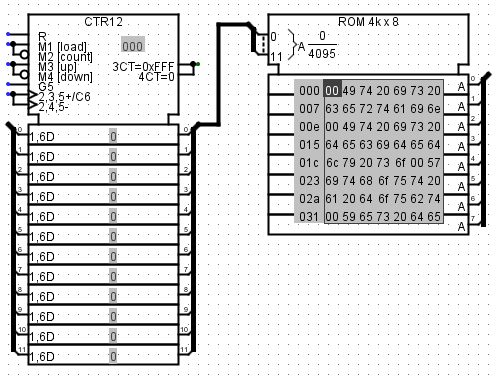
\includegraphics[width=\maxwidth{.95\linewidth}]{gfx/09-03}
	\caption{ROM Filter Mux}
	\label{fig:09-03}
\end{figure}

A five-bit Random Generator (\textit{Memory} library) is used to select a message at random. Figure \ref{fig:09-04} illustrates the placement of the random generator.

\begin{figure}[H]
	\centering
	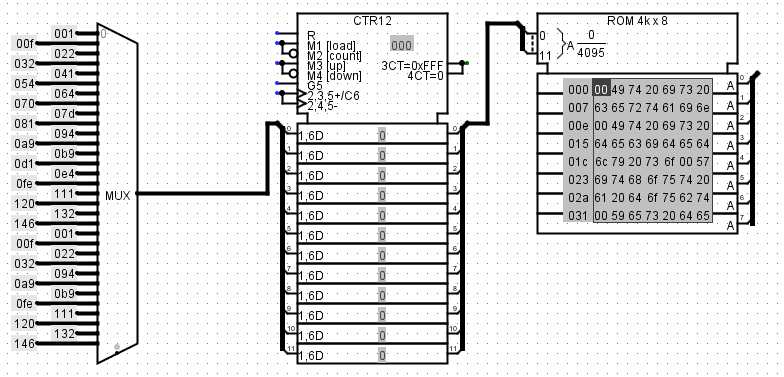
\includegraphics[width=\maxwidth{.95\linewidth}]{gfx/09-04}
	\caption{Random Generator Added}
	\label{fig:09-04}
\end{figure}

Next, a one-shot generator is added to the circuit. This is a simple subcircuit that is designed such that when activated it will output a high signal for a single clock pulse and then return to a low. In this circuit, when the reset signal goes high the first flip-flop changes so \textit{Q} is high. On the next clock pulse, the second flip-flop changes and \textit{Q} goes high. On the next pulse both flip-flops return to their quiescent state. The circuit has also added a clock that links to a Tunnel (\textit{Wiring} library) and then to the input of the one-shot. There are two other tunnels connected to the one-shot and they will be linked shortly.

\begin{figure}[H]
	\centering
	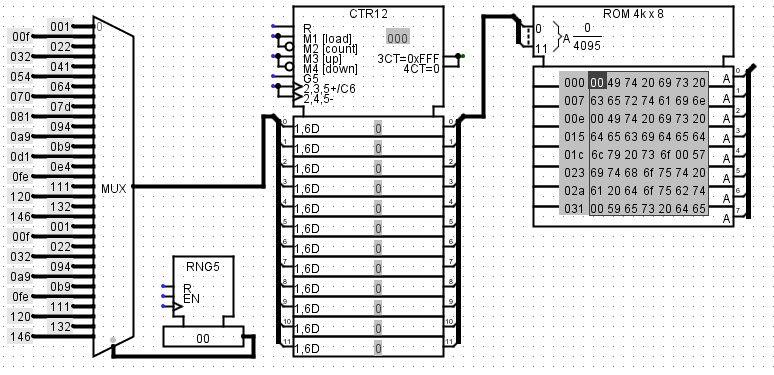
\includegraphics[width=\maxwidth{.95\linewidth}]{gfx/09-05}
	\caption{One-Shot Added}
	\label{fig:09-05}
\end{figure}

To complete the circuit, a few odds-and-ends were added.

\begin{itemize}
	\item Four signals were added to control the counter. Those signals are made available from tunnels and are actually generated elsewhere in the circuit.
	\item Tho signals were added to the one-shot subcircuit. The enable is linked through an \texttt{AND} gate to the clock of the random generator. Thus, whenever a reset signal is received the random generator will choose another 8-ball saying at random. Also, \textit{ttyClr} is generated to clear the teletype device on the \lstinline[columns=fixed]|main| circuit.
	\item The output of the ROM device is connected to the \textit{ttyOut} port in order to drive the teletype device on the \lstinline[columns=fixed]|main| circuit.
	\item Note that at the output of the ROM device is a splitter. ASCII letters are only seven bits wide so this splitter passes bits 0-6 to the \textit{ttyOut} port but bit 7 (the most significant bit) is simply discarded.
	\item Near the output of the ROM device, an \texttt{AND} gate feeds the \textit{ttyClk} signal, which is used on the \lstinline[columns=fixed]|main| circuit to clock the teletype device.
	\item The Bit Finder (\textit{Arithmetic} library) attached to the output of the ROM device is used to find the lowest-order one in the ROM byte. If the ROM byte includes at least one one then the south port is high but it goes low if the ROM byte is all zeros. That is the \textit{ena} signal that enables the clock and, when it goes low, permits a \textit{rst} signal (generated on the \lstinline[columns=fixed]|main| circuit when the user ``asks another question'') to create a new answer.
\end{itemize}

Figure \ref{fig:09-06} illustrates the complete Magic 8-Ball circuit.

\begin{figure}[H]
	\centering
	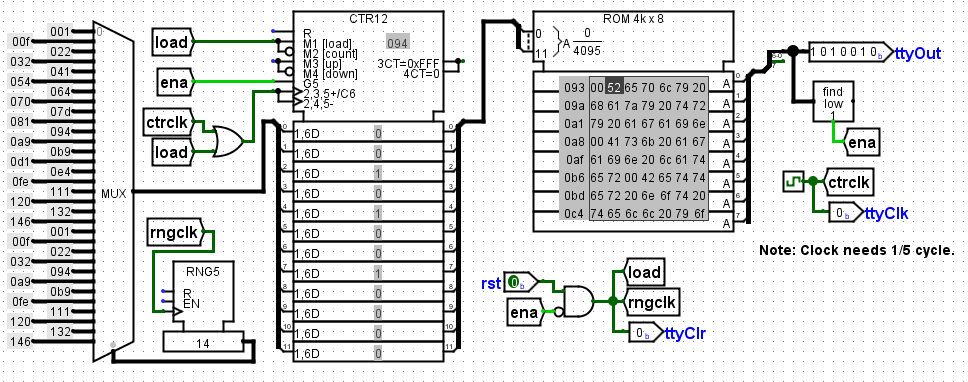
\includegraphics[width=\maxwidth{.95\linewidth}]{gfx/09-06}
	\caption{Complete Magic 8-Ball Circuit}
	\label{fig:09-06}
\end{figure}

The only remaining step is to create the \lstinline[columns=fixed]|main| circuit. As in all labs in this manual, the \lstinline[columns=fixed]|main| circuit does nothing more than provide a user interface for the Magic 8-Ball Circuit. Figure \ref{fig:09-07} illustrates the \lstinline[columns=fixed]|main| circuit.

\begin{figure}[H]
	\centering
	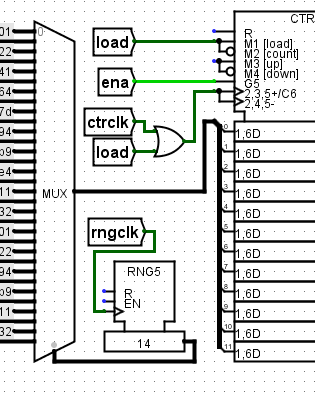
\includegraphics[width=\maxwidth{.95\linewidth}]{gfx/09-07}
	\caption{Magic 8-Ball Main Circuit}
	\label{fig:09-07}
\end{figure}

\subsection{Testing the Circuit}

Before the circuit can be tested the ROM device must be loaded. The ROM was loaded earlier in the lab but in case it does not have any content (it is filled with zeros), then load it with \emph{\texttt{Lab09\_ROM.txt}}, which was provided with the lab. To load the ROM device, click it one time and then click the ``(click to edit)'' link in its properties panel. In the ROM editor window that pops up, click the ``open'' button and find the ROM memory file. Click ``close window'' to load the ROM device and make it ready for service.

The circuit should be tested by enabling the simulator clock at a frequency of 16K Hertz. Every time the \textit{Reset} button is pressed a new random message will be displayed on the teletype screen.

\section{Deliverable}

To receive a grade for this lab, build this circuit. Be sure the standard identifying information is at the top left of the \lstinline{main} circuit, similar to: 

\bigskip
% The minipage environment keeps the three lines together - no page break.
\begin{minipage}{\linewidth}
	\begin{verbatim}
	George Self
	Lab 09: ROM
	February 16, 2018
	\end{verbatim}
\end{minipage}
\bigskip

Save the file with this name: \textit{Lab09\_ROM} and submit that file for grading.

